\section{Methods}
\label{sec:methods}
This sections describes the most important software design decission of this experiment e.g. how a fault tolerant Chandy Misra algorithm can be implemented or how I simulate faults.
Later, I describe the software and machines used.
\subsection{Chandy Misra}
- src Distributed algorithms by Fokking
- either write and connec this ro just reference this in the next chapter
\subsection {Fault tolerant Chandy Misra}
\label{ssec:fault-tolerant-chandy-misra}
The fault-tolerant Chandy Misra version used for our experiments constructs a sink tree in an undirected network under the assumption that a perfect failure detector is present at each node (a detector that does not suspect nodes that haven't actually failed and detects each failure eventually). 
Other than the original Chandy Misra algorithm, the fault tolerant version requires FIFO-channels.
Furthermore, I assume that the root node cannot fail because otherwise there is no sink tree to construct.

As far as Chandy-Misra is concerned nodes are only interested in crashes of their parents and other ancestors on their path to the root node.
If a node \co{X} detects a crash of its parent, it sends a \co{REQUEST} message to each neighbour. 
If a neighbour \co{Y} of \co{X} receives a \co{REQUEST} message, it answers with a \co{DIST d} message where \co{d} is its own distance. 
To save messages \co{DIST d} is only send if $d < \infty $.
If \co{Y} happens to be a child of \co{X}, it resets its own \co{dist} and \co{parent} value to $\infty$ respectively $\bot$ and sends a \co{REQUEST} message to all its neighbours. In this case \co{Y} sends no \co{DIST} message as answer to \co{X}.

The requirement for FIFO channels is best understood by a counterexample example based on a none FIFO network.
The network used for this example is shown in \cref{fig:fifoNecessaryNetwork}. 
Only important messages are mentioned; all others can be assumed to be send and received in any order.
The Chandy Misra algorithm starts with \co{A} as root node sending \co{DIST 0} messages to \co{B} and \co{C} which on receive consider \co{A} there parent and update their \co{dist} variable.
They also send \co{DIST} messages to their neighbours. 
When \co{C} and \co{D} receive the \co{DIST} messages from \co{B} respectively \co{C} they consider \co{B} respecitively \co{C} their parents.
\co{C} sends a \co{DIST 2} message to \co{D} - lets call it \co{M1}.
Now \co{B} crashes and when \co{C} detects this, it sends a \co{REQUEST} message towards \co{A} and \co{D} - call the latter \co{M2}.
If \co{M2} overtakes \co{M1}, \co{D} resets its variabbles and on receive of \co{M1} considers \co{C} its parent which is correct but with an incorrect \co{dist} value of 2.
All \co{DIST} messages received by \co{D} from now on have a higher distance value and are dismissed. 
So the error is never corrected.

A straightforward fix for this is to use FIFO networks because the original problem is that \co{M2} overtook \co{M1}.

SafraFT uses the same FIFO channels as its basic algorithm during the experiment.
Nonetheless, we still claim it does not need this property.
This claim is straightforward to proof: SafraFT guarantees that at most one message is in any channel at all times because it forwards a single token and when a backup token is issued, it is sent to a different node than the original token and only the first of both tokens are forwarded afterwards.
Following the reasoning that only one message is in flight between any two nodes, SafraFT is indifferent to the property FIFO property of the channels.

\begin{figure}[h]
	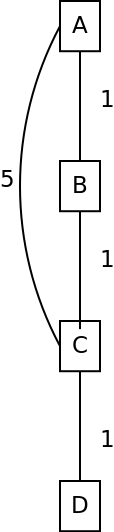
\includegraphics[height=5cm]{figures/FIFO_necessary}
	\centering
	\caption{None FIFO network with \co{A} as root to demonstrate necessity of FIFO networks.}    
	\label{fig:fifoNecessaryNetwork}
\end{figure}

I argue the this augmented Chandy Misra algorithm constructs correct sink trees in presence of fail-safe failures. 
Each failure only affects nodes that see themselves as children, grandchildren or deeper ancestor of the crashing node; that is, a failure only affects subtrees.
The children eventually send \co{REQUEST} messages to all their neighbours because the perfect failure detector guarantees that each node failure is eventually detected by them.
The neighbours send \co{REQUEST} messages to all their neighbours if they receive a \co{REQUEST} message from their parent. 
Therefore, eventually, all nodes in the subtrees of a failing node are reached by a \co{REQUEST} message and reset their \co{dist} and \co{parent} values.
Also, all neighbours that receive a \co{REQUEST} message from a node that is not their parent, answer it with their current \co{dist} value.
This allows nodes in the affected subtree to rebuild new paths toward the root node.
These new paths are correct when the answering node is not part of any affected subtree.
However, if they are part of an affected subtree (e.g. grandchildren of the crashed nodes), invalid paths are introduced - as these nodes might have not been reached by any \co{REQUEST} message and therefore still believe they have a valid path towards the root.
These invalid paths are corrected when the grandchildren are reached by the \co{REQUEST} message of their parent because on the receipt they send \co{REQUEST} messages which reset all nodes considering them parents. 
This behaviour of introducing invalid paths that are corrected later might lead to a bad theoretical message complexity but did not hinder the experiments.

The presented fault tolerant Chandy Misra algorithm could be incorrect as it calculated the wrong tree in 12 out of 1500, 
%number
Unfortunately, I could not fix it in time for the final experiment runs. 
However, this does not influence the evaluation of SafraFT because the correctness check for SafraFT and Chandy Misra in the experiment setup are designed to work independently from each other (see \cref{ssec:verification}).
The verification of SafraFT does show that SafraFT detected termination correctly in these cases and did not cause the corrupted Chandy Misra result.

Additionally, to fixing the last bugs, fault-tolerant Chandy Misra version could be improved by relieving the necessity for FIFO-channels, a more formal and adapted proof of correctness and a thorough complexity analysis. 

%TODO Provide pseudo code?
% TODO provide example?

\subsection{Fault Simulation}
I simulate faults by stopping Safra and the basic algorithm on the failing instance.
In particular, a crashed node does not send or react to tokens or basic messages.
Faults are triggered before and after interesting events e.g. directly before or after sending a basic message or token. 
Before every experiment run it is determined at random which node is going to fail, on which event it is going to fail and after how many repetitions of this event e.g. after the 3rd time it forwards a token.

In particular, I selected the following events to trigger a crash if not specified differently the crash is triggered before or after the event:
\begin{itemize}
	\item sending a token (1 to 3 repetitions)
	\item sending a backup token (1 to 2 repetitions)
	\item before receiving a token (1 to 3 repetitions)
	\item sending a basic message (1 to 5 repetitions)
\end{itemize}
The range of repetitions is limited to maximize the chance that a node meant to fail actually does so. 
However, a node that is planned to fail is not guaranteed to do so.
For example, this leads to runs where 90\% of the nodes should fail but only 88\% do so.
I verify for every run that the number of crashed nodes does not vary more than 10\% from the expected number. For runs with only 1 to 5 failing nodes, I confirm that at least one instance failed.

Alternatively, to the chosen approach to trigger failures, I considered the more random mechanism of running a thread that kills an instance after a random amount of time.
One could argue that this would be more realistic.
However, I believe this kind of an approach leads to less interesting failures because the vast majority of these failures would occur during idle time. 
Furthermore, most failures between internal events are observed as exactly the same on all other nodes. 
For example, other nodes cannot observe if a failure happened before an internal variable changed or after. 
In fact, they can only observe a difference when the failure happens after or before sending a message to them.
Hence, I have chosen a fault mechanism that focusses on these distinguishable scenarios.
As one might notices, the failure points are chosen to give rise to many different situations for our Safra version to deal with. 
I deliberately decided against choosing special failure points with regard to the basic algorithm because this would lead to less focused testing of the fault tolerance of Safra.

\subsection{Fault Detection}
Our Safra version assumes the presence of a perfect fault detector.
This kind of fault detection is easy to implement and integrate with the system e.g.
\cite{Fokkink:2018} on page 113 describes a straightforward implementation.

As building a perfect fault detector is a well known and solved problem, but nonetheless, time-consuming, I decided to avoid implementing one.
For this experiment, fault detection is simulated by sending \co{CRASH} messages from crashing nodes to their neighbours. 
These crash messages are send through different channels than basic and Safra messages because otherwise they would arrive in FIFO order with them and this would exclude situations where a basic messag is received after the crash of the sender has been detected.

\co{CRASH} messages are not broadcasted to all nodes because IBIS (the message passing library I used) does not provide broadcasting.  

\subsection{Offline Analysis}
\label{ssec:offline-analysis}
For the experiment, I measure some metrics before and after termination e.g. the total token count and tokens sent after termination of the basic algorithm.
To allow generation of these metrics, I need a close estimate of when the basic algorithm terminated.
For this, I generate log files of events during execution and analyse these afterwards.

Termination is commonly defined by:
\begin{enumerate}
	\item All nodes are passive
	\item No messages are in the channels
\end{enumerate}
To allow verification of 1. every node logs changes of its active status.
The second point can be verified indirectly by logging all changes of the message counters managed by Safra's algorithm.
These counters are incremented for each message sent and decremented when a message is received.
Therefore, one can conclude that no messages are in flight when the sum of all counters is 0.
All nodes log the aforementioned events combined with a timestamp.
By sorting and keeping track of active statuses, as well as, the sum of message counters, one can estimate the time of basic termination by the timestamp of the last node becoming passive while the sum of all message counters is zero.
This technique is similar to the one Safra uses but a global view on the system achieved by offline analysis allows to detect the time of basic termination more closely.

With this system in place, it is possible to determine the number of tokens sent after termination by logging each token sent event and categorizing them during the offline analysis.

Processing time metrics are determined by the same principle: processing time is logged online and is grouped into total and after termination by analysing the logs after the run.
Wall time between basic termination and detection by Safra is determined by comparing the timestamp of the event causing termination with the timestamp of the to announce call by Safra.

\subsection{Environment}
This chapter describes software, hardware and simulated network topology used for the experiments.
\subsubsection{IBIS}
IBIS is a Java-based platform for distributed computing developed by researchers of the Vrije Universiteit Amsterdam. 
Its subpart IPL is used as the message passing library for this project. 
I use version 2.3.1 which can be found on GitHub: \href{https://github.com/JungleComputing/ipl/releases/tag/v2.3.1}{https://github.com/JungleComputing/ipl/releases/tag/v2.3.1}.

Communication channels in IPL are backed by TCP and provide asynchronous messaging.
For this experiments, I also used IPL's ability to guarantee FIFO channels.
\subsubsection{DAS 4}
The experiment is conducted on the part of DAS-4 that belongs to the Vrije Universiteit Amsterdam. 
The nodes use primarily SuperMicro 2U-twins with Intel E5620 CPUs and a Linux CentOS build with the kernel version 3.10.0-693.17.1.el7.x86\_6.
For communication 1Gbit/s Lan is used.
At the time of the experiments, the VU had 41 nodes with 8 cores each.
Therefore, multiple instances were run on each physical node to be able to test our algorithm on decent sized networks (the number of machines and instances per machine can be found in \cref{table:runs}).
This is possible because Safra and Chandy Misra are both communication heavy with rather low processing and memory requirements.

\subsubsection{Network Topology}
Chandy Misra needs a network topology to work on. 
It requires an undirected network.
To generate more interesting runs I use weighted networks.

Our Safra version needs an undirected ring. 
For simplicity in my setup, this ring is part of the network the basic algorithm runs on. 
That means there is always an undirected ring connecting all nodes within simulated networks.

All networks for the experiments are generated by choosing randomly between 1 and 5 neighbours for each node and assigning a random, unique weight between 1 and 50000 to each channel.

After this channels with the heavy weight of 400000 are added between the root and some nodes to ensure the network stays connected when nodes fail.
For this, I calculate the expected network with knowledge of the nodes predetermined to fail and add connections between nodes that could become disconnected as some other nodes fail and the root.
These channels are heavyweight to avoid using them over `regular' channels which might create highly similar topologies with a lot of nodes directly connected to the root.

At last, channels are added to form an undirected ring in which each channel has the weight of 100000. 
Again the weight is chosen to avoid `overusing' the ring channels for the trees built.

For the experiments, I am not interested in the relationship between network topology and the measured metrics because this kind of analysis seems too detailed to show the correctness of our Safra version or to compare
our Safra version with the traditional Safra version.
Therefore, the exact network topology is not recorded. 
Anyhow, I output the depth of resulting trees and the nodes per level for runs up to 500 nodes.
This information is recorded to allow for quality checks and ensure the experiments were not run on trivial networks.
Generating these statistics for runs with over 500 nodes turned out to be time-consuming.
Hence, I decided not to generate them.
However, if the network topology leads to none trivial, deep trees for 500 nodes and less, it seems highly unlikely that it would not for even more nodes.
Furthermore, I verified that the topology generated for more than 500 nodes still leads to interesting cases by spot sample.

